\documentclass{article}

\usepackage{times}
\usepackage[top=1in, bottom=1in, left=1in, right=1in]{geometry}
\usepackage{graphicx}
\usepackage{float}

\floatstyle{ruled}
\newfloat{program}{thp}{lop}
\floatname{program}{Program}

\begin{document}

\author{Joshua Ashby\\
\\
        Linux And Sci\\
                \texttt{http://joshashby.com}\\
		\texttt{joshuaashby@joshashby.com}}
\title{ThreadGUI Doc}

\maketitle

\tableofcontents
\newpage
\abstract{ThreadGUI is a GUI system that is made to be easy to use and add on to. It builds the GUI in a second thread so the GUI does not have to mess with timing or sleep functions in the main thread and so on. It includes square buttons, circlular buttons, labels, bullet list items (single and dual line), lines, and single line text.}\\
\section{Introduction}
Writing ThreadGUI came to mind when I was working on programming a new GUI for my robot BOB. I had recently started to program a few projects in C++ again, and was getting the hang of using the Open Frameworks library. Seeing that I may want to use Open Frameworks, and the lack of GUI systems for it, I decided to write one my self.\\
\section{Setting up}
ThreadGUI uses the Open Frameworks C++ libraries, and comes packed with only the project files. as a result you'll have to download Open Frameworks FAT. after downloading and setting up, download all the files from the master branch of ThreadGUI from here:\\
git clone git://github.com/JoshAshby/ThreadGui.git\\
Place (or clone) these files into a file in the Open Frameworks apps/myApps directory. For example, if my user was Joe then it might look like this:\\
/home/joe/openframeworks/apps/myApps/threadgui\\
Now your ready to start working with ThreadGUI.\\
\section{testApp.cpp/.h}
There are two files that, if you just want to use ThreadGUI out of the box, you have to change/write. When you browse through the src file, you'll see theres four files. For those of you that are familiar with Open Frameworks you'll know that main.cpp doesn't need edited unless you want to change the screen settings. testApp.cpp holds an example of all the different functions that are included in ThreadGUI. For example: Program \ref{code1}\\
\begin{program}
\begin{verbatim}
TO.roundButtonGreen(400,400,20,"Hello",1);
\end{verbatim}
\caption{Example of the format used}
\label{code1}
\end{program}\\
TO is the main ThreadGUI function. If you look at testApp.h you'll see two lines of code that looks like so:\\
\begin{program}
\begin{verbatim}
#include "threadedObject.h"
...
threadedObject	TO;
\end{verbatim}
\caption{testApp.h}
\label{code2}
\end{program}\\
This is where you can change the call name if you don't want to use TO.
\section{threadedObject.h}
This is the main ThreadGUI file, where all of the functions to draw the GUI are. 
\subsection{buttonAction(int button);}
In this function is where you define what all the buttons will do, by button number in a case structure.
\subsection{threadedObject();}
Here you can set variables to different values.
\subsection{start();}
Starts the ThreadGUI thread
\subsection{stop();}
Stops the ThreadGUI thread
\subsection{threadedFunction();}

\subsection{label(int x, int y, char str[20]);}
This creates a label at (x,y). the width is determined by the length of str[], and the height is always set at 20px.\ref{label}\\
\begin{figure}[htp]
  \begin{center}

\includegraphics[]{label}
  \end{center}
  \caption{Normal label}
\label{label}
\end{figure}\\

\subsection{labelGreen(int x, int y, char str[20]);}
Same as above but green colored.\ref{labelgreen}\\
\begin{figure}[htp]
  \begin{center}

\includegraphics[]{labelgreen}
  \end{center}
  \caption{Green label}
\label{labelgreen}
\end{figure}\\

\subsection{labelGrey(int x, int y, char str[20]);}
Same as above but grey colored.\ref{labelgrey}\\
\begin{figure}[htp]
  \begin{center}

\includegraphics[]{labelgrey}
  \end{center}
  \caption{Grey label}
\label{labelgrey}
\end{figure}\\

\subsection{rectButton(int x, int y, char srt[15], int color);}
Creates a square button with the center at (x,y), with the text in srt[]. The width and height are automatically calculated from the length of srt[].\ref{rectbutton}\\
\begin{figure}[htp]
  \begin{center}

\includegraphics[]{rectbutton}
  \end{center}
  \caption{Normal rectButton}
\label{rectbutton}
\end{figure}\\

\subsection{rectButtonGrey(int x, int y, char srt[15], int color);}
Same as above but grey colored.\ref{rectbuttongrey}\\
\begin{figure}[htp]
  \begin{center}

\includegraphics[]{rectbuttongrey}
  \end{center}
  \caption{Grey rectButton}
\label{rectbuttongrey}
\end{figure}\\

\subsection{rectButtonGreen(int x, int y, char srt[15], int color);}
Same as above but green colored.\ref{rectbuttongreen}\\
\begin{figure}[htp]
  \begin{center}
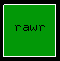
\includegraphics[]{rectbuttongreen}
  \end{center}
  \caption{Green rectButton}
\label{rectbuttongreen}
\end{figure}\\

\subsection{roundButton(int x, int y, int h, char srt[15], int color);}
Creates a circlular button with the center at (x,y) with radius h and text srt[].\ref{roundbutton}\\
\begin{figure}[htp]
  \begin{center}

\includegraphics[]{roundbutton}
  \end{center}
  \caption{Normal roundButton}
\label{roundbutton}
\end{figure}\\

\subsection{roundButtonGrey(int x, int y, int h, char srt[15], int color);}
Same as above but grey colored.\ref{roundbuttongrey}\\
\begin{figure}[htp]
  \begin{center}

\includegraphics[]{roundbuttongrey}
  \end{center}
  \caption{Grey roundButton}
\label{roundbuttongrey}
\end{figure}\\

\subsection{roundButtonGreen(int x, int y, int h, char srt[15], int color);}
Same as above but green colored.\ref{roundbuttongreen}\\
\begin{figure}[htp]
  \begin{center}

\includegraphics[]{roundbuttongreen}
  \end{center}
  \caption{Green roundButton}
\label{roundbuttongreen}
\end{figure}\\

\subsection{click(int x, int y);}
calculates which button has been clicked then passes that button to buttonAction.\\

\subsection{click(int color);}
Same as above, but only the button number is passed to it. This could be used for key presses.\\

\subsection{line(int x,int y, int xc, int yc, int thick);}
Creates a white line from point (x,y) to (xc,yc) with the thickness thick.\ref{line}\\
\begin{figure}[htp]
  \begin{center}

\includegraphics[]{line}
  \end{center}
  \caption{Normal line}
\label{line}
\end{figure}\\

\subsection{lineGreen(int x,int y, int xc, int yc, int thick);}
Same as above but green colored.\ref{linegreen}\\
\begin{figure}[htp]
  \begin{center}

\includegraphics[]{linegreen}
  \end{center}
  \caption{Green line}
\label{linegreen}
\end{figure}\\

\subsection{lineGrey(int x,int y, int xc, int yc, int thick);}
Same as above but grey colored.\ref{linegrey}\\
\begin{figure}[htp]
  \begin{center}

\includegraphics[]{linegrey}
  \end{center}
  \caption{Grey line}
\label{linegrey}
\end{figure}\\

\subsection{lineBlue(int x,int y, int xc, int yc, int thick);}
Same as above but blue colored.\ref{lineblue}\\
\begin{figure}[htp]
  \begin{center}

\includegraphics[]{lineblue}
  \end{center}
  \caption{Blue line}
\label{lineblue}
\end{figure}\\

\subsection{bullet(int x, int y, char str[20]);}
Creates a bulleted list item with the top corner at (x,y) and the text str[].\ref{bullet}\\
\begin{figure}[htp]
  \begin{center}

\includegraphics[]{bullet}
  \end{center}
  \caption{Normal bullet}
\label{bullet}
\end{figure}\\

\subsection{bulletGreen(int x, int y, char str[20]);}
Same as above but green colored.\ref{bulletgreen}\\
\begin{figure}[htp]
  \begin{center}

\includegraphics[]{bulletgreen}
  \end{center}
  \caption{Green bullet}
\label{bulletgreen}
\end{figure}\\

\subsection{bulletBlue(int x, int y, char str[20]);}
Same as above but blue colored.\ref{bulletblue}\\
\begin{figure}[htp]
  \begin{center}

\includegraphics[]{bulletblue}
  \end{center}
  \caption{Blue bullet}
\label{bulletblue}
\end{figure}\\

\subsection{mlBullet(int x, int y, char str[20]);}
Same as a regular bullet, but this allows for the text to use up 2 lines instead of 1.\ref{mlbullet}\\
\begin{figure}[htp]
  \begin{center}

\includegraphics[]{mlbullet}
  \end{center}
  \caption{Normal mlBullet}
\label{mlbullet}
\end{figure}\\

\subsection{mlBulletGreen(int x, int y, char str[20]);}
Same as above but green colored.\ref{mlbulletgreen}\\
\begin{figure}[htp]
  \begin{center}

\includegraphics[]{mlbulletgreen}
  \end{center}
  \caption{Green mlBullet}
\label{mlbulletgreen}
\end{figure}\\

\subsection{mlBulletBlue(int x, int y, char str[20]);}
Same as above but blue colored.\ref{mlbulletblue}\\
\begin{figure}[htp]
  \begin{center}

\includegraphics[]{mlbulletblue}
  \end{center}
  \caption{Blue mlBullet}
\label{mlbulletblue}
\end{figure}\\

\subsection{text(int x, int y, float data);}
This ones a little decieving, as it really is a data function, in the ThreadGUI-BOB-GUI branch, this has been renamed to dataFloat. Simply this function takes and places formated text at (x,y+4). The y+4 is so the same coordinates can be used with the bullets and have the text line up still.\ref{text}
\begin{figure}[htp]
  \begin{center}

\includegraphics[]{text}
  \end{center}
  \caption{Text}
\label{text}
\end{figure}\\

\end{document}
